\chapter{Introduction v2.0}
\setcounter{section}{0}
%%%%%%%%%%%%%%%%%%%%%%%
\textit{Changelog:}\\
\begin{itemize}
	\item \textit{v2 \textbf{\diffdate{2024}{06}{18}{2024}{06}{24}}. The thought of a rubric came when working on the third rubric: Leadership.}
	\item \textit{v1 unclear}
\end{itemize}
%%%%%%%%%%%%%%

\section{Meaning of a Rubric} \label{sec:Rubric}
\paragraph{Coherent Decision Framework}

A rubric for a given topic is a collection of principals, goals or a thesis under a \gls{p_CDF}.\\

The process of integrating items of a rubric under \gls{p_CDF} also defines the topic itself. Since there is no natural boundary where a topic can end, defining these boundaries is part of the process of developing a rubric.\\

In this context, \textit{coherent} means that the parts of the rubric are connected with each other. The process involves testing parts of the rubric against each other to ensure they are:
\begin{description}
    \item[Aligned] supporting the main topic's goals or thesis.
    \item[Non-Contradictory] not in contradiction with other parts; if contradictions exist, the rubric should address how to resolve them.
    \item[Integrated] ideally, many parts of the decision framework should be integrated with each other, thereby reinforcing alignment towards the goal or thesis.
\end{description}

\paragraph{Communicated clearly and consistently:}
To handle the complexity of the created structure, a quality criterion is that a \textit{rubric} must be communicated clearly and consistently.

\paragraph{Relationship between a Strategy}

Loosely speaking, a strategy is a rubric plus specific actions (Maßnahmen).

The \textit{main two differences} are:
\begin{itemize}
	\item A strategy contains \textit{specific actions/ decision (Maßnahmen/ Entscheidungen)} that are already decided to be taken.
	\item It is more strict in defining the boundaries of a topic. The analysis of the \textit{playing field} assesses the topic or playing field against other actors.
\end{itemize} 

A strategy outlines specific actions based on set goals and analyzes them and the game field where they should play out. A rubric provides a coherent framework to make choices along the line. Along those lines, a strategy can contain the same elements as a rubric. These are then integrated into a \gls{p_CDF} for continuity.

\section{Strategie} \label{Appendix_Erlaeuterung_Strategie}
\subsection{Erläuterung}
\paragraph{Definition}
Eine Strategie besteht aus einer Menge aus \textit{integriert} Entscheidungen, welche einem auf einem Spielfeld bestmöglich für einen Erfolg positioniert.\\

% Stategy - A integrated set of choices, which position you on a playing field of you choice to win.

%% Theory: This theory has to be coherent and doeable.:
%%% Why are we on this playing field on not on a other one.
%%% How we are on this playing field better the anyone else on serving the customer.

%% Difference to planing: To coherent structure is nessesary. In planing, you choice activity where the outcome is determinde by you. The strategy makes prediction about what we are going to to to archive a certain outcome.

\begin{figure}[H]
	\centering
	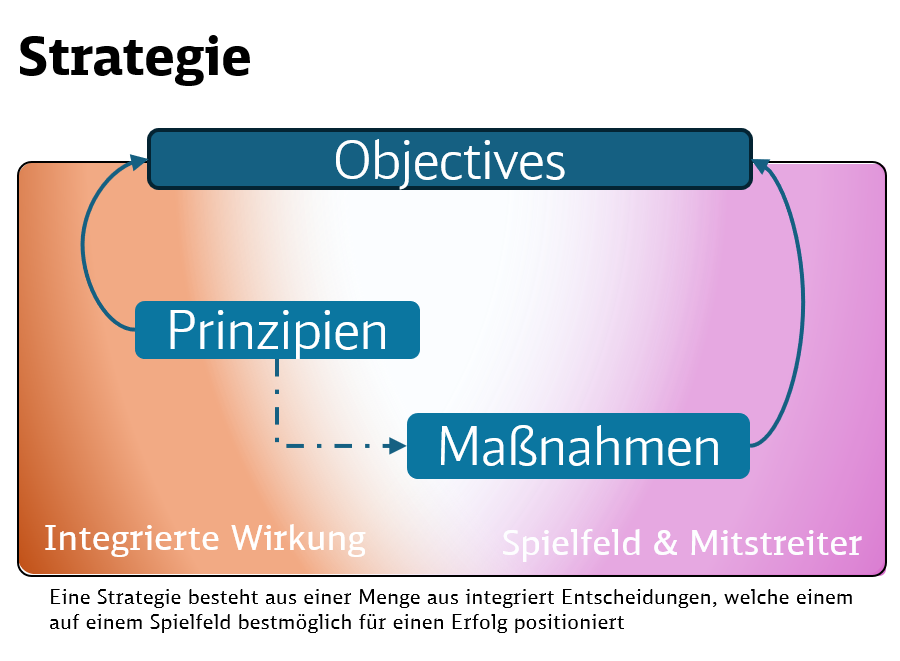
\includegraphics[scale = 0.3]{attachment/chapter_OWN/Scc006.png}
	\caption{Skizze Konzept Strategie}
\end{figure} 

\paragraph{Integrierte Maßnahmen/ Entscheidungen (Decision/ Action)} sind Entscheidungen, die von einer kohärenten Theorie geleitet werden, die erklärt, warum und wie sie einen bestmöglichen Nutzen bringen werden. Dabei kann auf vorhandene Wirkungszusammenhänge zurückgegriffen oder angenommene genutzt werden, die später überprüft werden. Um das Spielfeld oder die Umgebung, den Markt, einzuschätzen, ist eine Analyse erforderlich. Dabei sollen die Regeln, Chancen und Risiken identifiziert werden, die für das Handeln relevant sind. Ebenso ist es wichtig zu erkennen, welche Wettbewerber ähnliche Zielsetzungen verfolgen und ob sie denselben Restriktionen unterliegen.

\paragraph{Unterschied zum Plan:} Ein Plan erfordert keine kohärente Struktur, die die Entscheidungen an einem Ziel ausrichtet oder erklärt, warum genau diese Entscheidung letztendlich zum Erfolg führen wird. Es kann sein, dass die Entscheidungen genau die gleichen sind, die auch durch eine überlegte Strategie getroffen worden wären. Eine Strategie ist jedoch selten statisch, und es erfordert Anpassungen der Strategie, wenn neue Informationen auftauchen. Zum Beispiel sind die Annahmen über das Spielfeld möglicherweise nicht vollständig oder korrekt. Jetzt zeigt sich der Vorteil einer Strategie im Vergleich zu einem Plan. Eine Strategie legt nahe, warum genau die Entscheidungen basierend auf den Gegebenheiten des Spielfelds getroffen wurden. Ändern sich die Gegebenheiten, so kann die Wirkung der Entscheidungen neu analysiert werden.

\subsection{Arten der Entscheidung}


\paragraph{Maßnahme} wird hier definiert als ein

\begin{itemize}
	\item \textbf{konkreter},
	\item \textbf{expliziter} und
	\item \textbf{abgeschlossener} Schritt.
\end{itemize}

Im Zusammenhang mit der Strategie wird über eine Maßnahme entschieden: Eine Maßnahme kann ein Projekt, eine Software oder eine eigene Strategie sein. Wichtig ist dabei, zu erklären und offenzulegen, wie diese Maßnahme zum übergeordneten Ziel beiträgt. Je nach Detailgrad können dabei

\begin{itemize}
	\item die exekutiven Schritte aufgeführt werden, um die abgeschlossene Maßnahme zu erreichen,
	\item und eigene Ziele festgelegt werden, die die Maßnahme abschließend bewertbar machen.
\end{itemize}

In der Strategieplanung kann diese Substruktur wiederum auf die großen Ziele bewertet werden.

\paragraph{Prinzip: Hilfestellung für zukünftige Entscheidungen} \label{Rubic:Prinzip}

Wenn noch keine Entscheidungen bezüglich Maßnahmen getroffen werden können, kann das Werkzeug \textbf{Prinzip} zum Einsatz kommen.\\

Hierbei gilt die Definition einer Strategie ebenso. Werden bestimmte Prinzipien festgelegt, müssen sie ebenfalls in einen kohärenten Rahmen eingebaut werden, der erklärt, warum diese Prinzipien dabei helfen, auf die Ziele einzuzahlen - die Wirkungskette.\\

Wie bereits erläutert, geht es bei einer Strategie darum, integrierte $"$Handlungsentscheidungen$"$ zu treffen, die einen näher an das Ziel bringen. Diese können entweder bereits festgelegte Maßnahmen sein \underline{oder} Prinzipien, die in bisher unbekannten, aber erwartbaren Situationen eine Richtung vorgeben, wie in Zukunft entschieden werden soll, um die Ziele zu erreichen, oder um in Zukunft Maßnahmen festzulegen.

\paragraph{Objectives allein reichen manchmal aus, sind aber keine Strategie}

Das Ziel einer Strategie ist es, die gesetzten Ziele zu erreichen, indem integrierte Entscheidungen getroffen werden, die einen so positionieren, dass die Ziele bestmöglich erreicht werden. Es kann jedoch auch sein, dass die Ziele selbst als Ausrichtung für zukünftige Entscheidungen (z.B. Abwägungen) dienen können.\\

Damit wir von einer Strategie sprechen können, sollten wenigstens Zielkonflikte und -abhängigkeiten analysiert werden. Diese könnten jedoch auch die gleiche Wirkung haben - dass sie ausreichen, die jeweiligen Ziele zu erreichen.\\

Ein persönliches Beispiel: Für meine eigene Ausrichtung im Leben habe ich drei Ziele definiert. Zu diesen Zielen sind weder Maßnahmen noch tiefergehende Prinzipien festgelegt.

\section{Prinzip und Mechanismus}\label{Appendix_Erlaeuterung_Prinzip}

Prinzipien und Mechanismen sind eng miteinander verbunden, da Prinzipien oft die zugrunde liegenden Konzepte oder Ideen sind, die die Funktionsweise eines Mechanismus bestimmen.

Ein Mechanismus ist die konkrete Umsetzung oder die praktische Realisierung eines Prinzips. Das Prinzip legt fest, wie etwas funktionieren soll, während der Mechanismus die spezifische Art und Weise beschreibt, wie dies tatsächlich erreicht wird.

Zum Beispiel könnte das Prinzip der Schwerkraft besagen, dass alle Massen auf der Erde von der Gravitationskraft angezogen werden. Der Mechanismus, der dies umsetzt, könnte die Bewegung von Objekten durch die Krümmung der Raumzeit gemäß der Allgemeinen Relativitätstheorie sein.

In diesem Zusammenhang liefert das Prinzip den theoretischen Rahmen, während der Mechanismus die praktische Umsetzung oder Realisierung dieses Prinzips beschreibt.
